\chapter{面向微博的反讽识别}
\label{cha:exp_irony_det}

\section{本章引论}

社交媒体的发展对我们的语言体系带来了很大的影响,网络上出现了很多新颖的用词和句式,语言的表达方式越来越丰富,也越来越复杂。而反讽是在网络上常见的语言修饰手法之一, 这为反讽相关的研究带来了充足的数据基础。Henry Watson Fowler在《The King's English》一书中指出反讽的使用使得“表面意思和实际意思不同”。譬如一个人说“你这想法真有创意”,在字面意思上是对另一个人的赞同,但在特定背景下,如后接一句“你真相信这能实现吗”,那么发言者实际上可能暗示这个想法无法落地,表面上称赞为“有创意”,其实是指责这种想法不切实际。这在意图识别当中尤其重要,忽略反讽的使用会导致对内容的错误理解,而且这种理解是和真实意思截然相反的,因此识别出反讽的使用或许对相关的场景如情感识别、人机交互能起着正面的作用。

根据Joshi等人\cite{joshi2017automatic}对近年相关研究的总结,反讽识别可以大致分成基于规则的方法和基于机器学习的方法。基于规则的方法透过人工找出反讽中的语言规律,设计出对应的模式,然后在新样本中尝试识别出相应的模式出现。和机器学习方法对比,基于规则的方法优点在于无需模型训练,但要求研究员对反讽有充分的语言理解,设计的模式对样本的复盖程度决定了算法的识别能力。而随着近年深度学习快速发展,一些研究更专注于对词嵌入向量的使用以及人工神经网络的设计和选择。

国际比赛SemEval-2018的任务三\cite{van2018semeval}旨在促进英语微博中的反讽识别研究,其中包含了两个子任务。子任务一是二分类的反讽识别,需要识别微博是否有使用反讽。子任务二是四分类的反讽识别,是子任务一的拓展,除了判断微博是否包含反讽,反讽再细分成三个类别:基于相反语义的反讽 
、情景反讽、其他反讽。本章节中我们将基于SemEval-2018的任务三进行实验,采用比赛组织者提供的训练数据和测试数据,并透过和其他参赛系统进行比较来评估我们提出的框架的性能。

本章的内容安排如下。在章节\ref{sec:exp_irony_det_format}中,我们会基于章节\ref{sec:global_problem_analysis}首先给出当前问题的形式化表示。在章节\ref{sec:exp_irony_det_data}中我们再对具体实验数据进行观察,分析微博文本的特性以及各个反讽类别之间的不同。在章节\ref{sec:exp_irony_det_framework}中,我们会基于章节\ref{sec:global_framework}的框架给出我们对当前问题的系统框架。最后在章节\ref{sec:exp_irony_det_exp}给出实验的细节,以及对实验结果进行分析。

\section{形式化表示}
\label{sec:exp_irony_det_format}

在本章中,我们要研究单条微博的反讽类型识别。给定一个反讽类别集合$C$,对于一个微博集合$T$,对任意一条微博$t \in T$,它属于唯一一种情感类别$c \in C$。又给定一个词集合$W$,微博$t$经过文本预处理后可以表示为一个长度为$L$的词序列 $w = <w_1, w_2, ..., w_L>, w_i \in W, i \in [1, L]$。因为没有引入上下文信息,所以背景$B$在模型中忽略。那么我们的目标是找出一个映射关系$F_C$,使得$c=F_C(w)$。

\section{数据观察}
\label{sec:exp_irony_det_data}

我们的实验完全采用SemEval-2018的任务三比赛组织者提供的数据集,其中的语料收集自微博平台Twitter上发布于2014年至2015年之间的微博,再由人工标注得出每条微博的反讽类型。该比赛的两个子任务均采用了相同的语料但标注稍有不同。子任务一是二分类的反讽识别,需要识别微博是否有使用反讽,各类别的数据分布如表\ref{tab:semeval_2018_task3_A_data}所示,表\ref{tab:semeval_2018_task3_A_sample}为语料中两个类别的例子。可以看出没有反讽和带有反讽两个类别的样本在训练集上大致比例为1:1,在测试集上两个类别的分布大致为3:2。

\begin{table}[htb]
  \centering
  \begin{minipage}[t]{0.7\linewidth} % 如果想在表格中使用脚注,minipage是个不错的办法
  \caption{反讽识别子任务一各类别样本数量分布}
  \label{tab:semeval_2018_task3_A_data}
    \begin{tabularx}{\linewidth}{X|XX}
    \toprule[1.5pt]
    数据集 & 没有反讽 & 带有反讽 \\  
    \hline
    训练集 & 1923 & 1911 \\
    测试集 & 473  & 311 \\
    \bottomrule[1.5pt]
    \end{tabularx}
  \end{minipage}
\end{table}

\begin{table}[htb]
  \centering
  \begin{minipage}[t]{0.8\linewidth} % 如果想在表格中使用脚注,minipage是个不错的办法
  \caption{反讽识别子任务一样例}
  \label{tab:semeval_2018_task3_A_sample}
  \begin{tabularx}{\linewidth}{l|X}
    \toprule[1.5pt]
    反讽类别 & 例子 \\
    \hline
    没有反讽 & Had no sleep and have got school now \#not happy \\
    带有反讽 & I just love when you test my patience!! \#not \\
    \bottomrule[1.5pt]
  \end{tabularx}
  \end{minipage}
\end{table}

子任务二是四分类的反讽识别,是子任务一的拓展,除了判断微博是否包含反讽,反讽再细分成三个类别:基于相反语义的反讽、情景反讽、其他反讽。各类别的数据分布如表\ref{tab:semeval_2018_task3_B_data}所示,表\ref{tab:semeval_2018_task3_B_sample}为语料中各反讽类别的例子。可以看出带有反讽一类细分成三个子反讽类别后各个类别的分别变得明显的不均匀,三个子反讽类别中的样本数据量差异也较大,基于相反语义的言语反讽占了其中一半以上,在模型训练过程应有对应策略处理。

\begin{table}[htb]
  \centering
  \begin{minipage}[t]{\linewidth} % 如果想在表格中使用脚注,minipage是个不错的办法
  \caption{反讽识别子任务二各类别样本数量分布}
  \label{tab:semeval_2018_task3_B_data}
    \begin{tabularx}{\linewidth}{X|XXXX}
    \toprule[1.5pt]
    数据集 & 没有反讽 & 基于相反语义的反讽 & 情景反讽 & 其他反讽\\  
    \hline
    训练集 & 1923 & 1390 & 316  & 205 \\
    测试集 & 473  & 164  & 85  & 62 \\
    \bottomrule[1.5pt]
    \end{tabularx}
  \end{minipage}
\end{table}

\begin{table}[htb]
  \centering
  \begin{minipage}[t]{\linewidth} % 如果想在表格中使用脚注,minipage是个不错的办法
  \caption{反讽识别子任务二样例}
  \label{tab:semeval_2018_task3_B_sample}
  \begin{tabularx}{\linewidth}{l|X}
    \toprule[1.5pt]
    \small 反讽类别 & 例子 \\
    \hline
    \small 没有反讽 & Had no sleep and have got school now \#not happy \\
    \small 基于相反语义的反讽 & \small I really love this year’s summer; weeks and weeks of awful weather \\
    \small 情景反讽 & Most of us didn’t focus in the \#ADHD lecture. \#irony \\
    \small 其他反讽 & @someuser Yeah keeping cricket clean, that's what he wants \#Sarcasm \\
    \bottomrule[1.5pt]
  \end{tabularx}
  \end{minipage}
\end{table}

比赛组织者对四种反讽类别给出了对应的说明。对基于相反语义的反讽一类,文本中存在某部分内容表达了可评估的情感极性,但整条微博实际上表达了相反的情感极性。如表\ref{tab:semeval_2018_task3_B_sample}中的例子,“love”在字面意思上表达了正面的情感,但微博后半中“awful weather”提示实际情况引起了发言者的不适,发言者其实在表达对这个夏天坏天气的不满,这和“love”的正面情感恰恰相反。对于情景反讽一类,文本正描述某个场景,其中发生的事情和某种预期不符。如表\ref{tab:semeval_2018_task3_B_sample}中的例子,描述了一个参与讲座的场景,但“我们(us)”并没有专注于这场讲座,和“参与者应该专注于讲座内容”的预期相反。对于其他反讽一类,文本表达了讽刺的意思,但文本的字面意思和发言者表达的意思之间并不存在情感极性的反差。如表\ref{tab:semeval_2018_task3_B_sample}中的例子,发言者表示某人想要保持蟋蟀干净,字面上并不存在情感极性,但在句子后的井号标签提示了发言者表达了讽刺,认为“保持蟋蟀干净”是一样莫名奇妙的事情。最后是没有反讽一类,对于明显不可能包含反讽的文本,或者在背景信息不足的情况下不能确认其包含反讽的文本均属于这一类。

\subsection{文本长度}

我们首先对数据集的文本经过简单分词后统计各个类别的样本中词数量的分布,以下简称为文本长度。表\ref{fig:semeval2018_task3_train_class_len}和表\ref{fig:semeval2018_task3_test_class_len}分别显示了训练集和测试集上各类别样本的文本长度。综合先见样本的文本长度不超过了50,样本的平均文本长度约为20个词。根据表\ref{fig:semeval2018_task3_train_class_len}我们可以看出“情景反讽”的样本整体的文本长度较其他类别的长,“没有反讽”和“基于相反语义的反讽”在文本长度分布上没有明显区别,“其他反讽”整体的文本长度则略高于前两者。再观察表\ref{fig:semeval2018_task3_test_class_len},同样地“没有反讽”和“基于相反语义的反讽”在文本长度分布上没有明显区别,“情景反讽”的文本长度略高于前两者,但不如训练集上明显。

\begin{figure}[H]
  \centering
  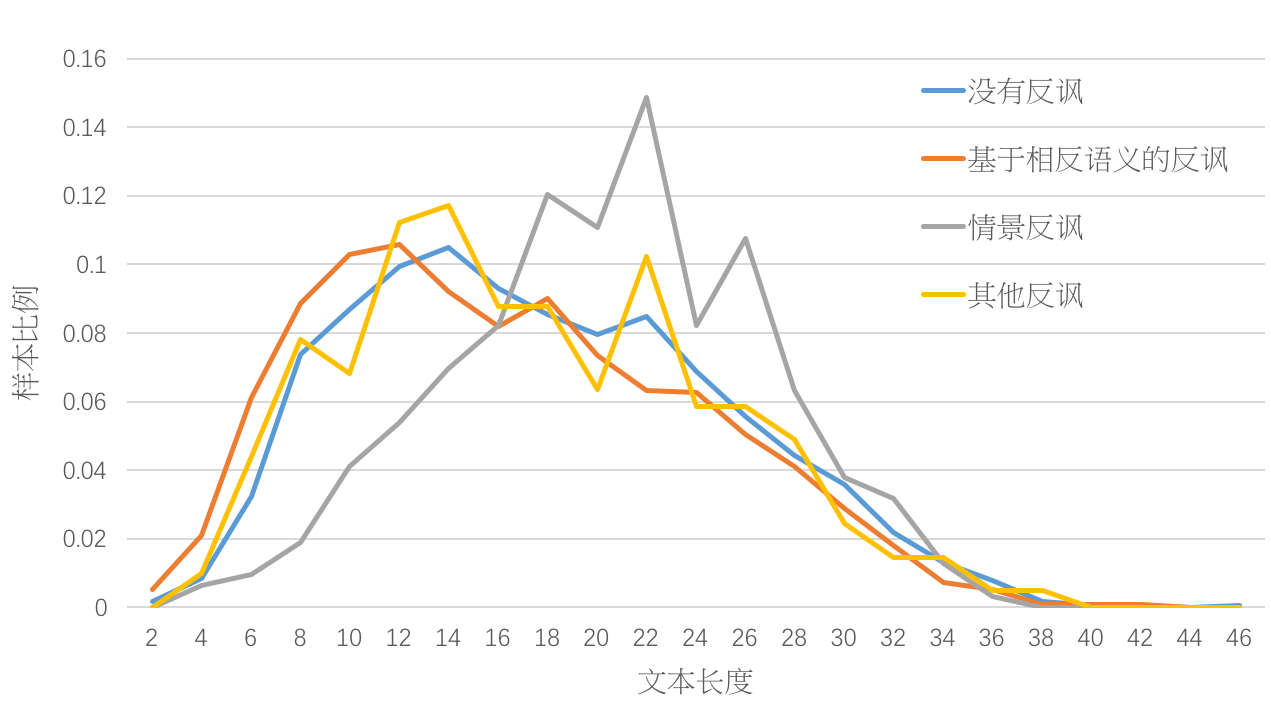
\includegraphics[width=\textwidth]{img/semeval2018_task3_train_class_len.png}
  \caption{反讽识别训练集上各类别文本长度分布}
  \label{fig:semeval2018_task3_train_class_len}
\end{figure}

\begin{figure}[H]
  \centering
  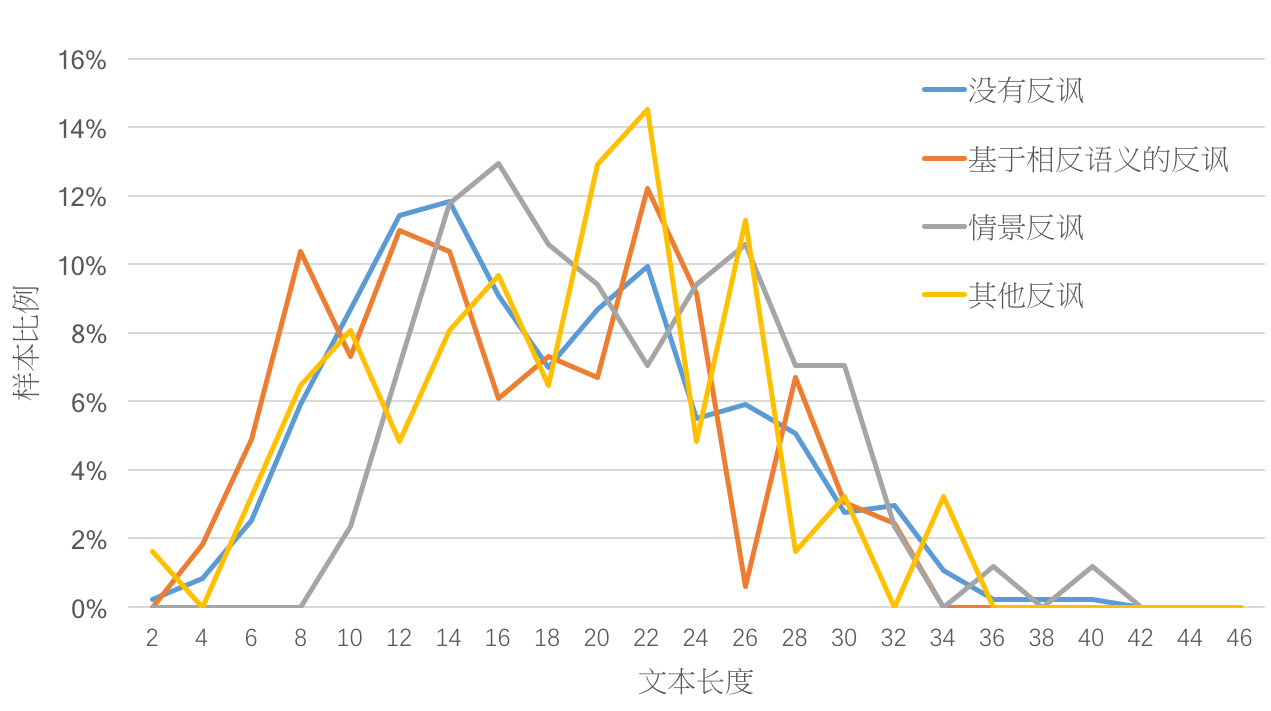
\includegraphics[width=\textwidth]{img/semeval2018_task3_test_class_len.png}
  \caption{反讽识别测试集上各类别文本长度分布}
  \label{fig:semeval2018_task3_test_class_len}
\end{figure}

\subsection{文本特征}
\label{ssec:exp_irony_det_data_text}

另外我们注意到语料中存在微博平台Twitter上特有的文本特征,出现频率较高的模式如下:

\begin{itemize}

\item 用户标签“@someuser”,对应微博上的一个用户,使用场景包括以下两种。一是作为句子中的名词使用,二是添加在句前或句末用于提示该用户的参与,不具有句法作用。

\item 井号标签“\#something”,使用场景大致分为以下两种。一是作为句子中的一部分,如“I \#do \#like \#it”,去除井号后满足正规的英语用法,此处以井号标签代替是对内容的强调。另一种是出现在句末,用于提示微博内容与标签对应内容相关,如句末出现“\#sarcasmtweet”明显表示讽刺。

\item 网站链接,在微博平台上支持附加一个网站链接以便,其中平台对链接进行了统一处理,在语料库中网站链接均形如“http://t.co/***”或“https://t.co/***”。

\item 转发标记“RT”(retweet),当用户转发某条微博并添加个人评论时,平台会自动在个人评论后附加转发的微博原文并以“RT”隔开。

\item 一些在社交媒体平台上常见的、有别于正规英语的用法,如拼写错误、缩略词、全大写字母的单词、表情符等,可以参考章节\ref{sec:text_preprocess}描述的例子。

\end{itemize}


\section{框架设计}
\label{sec:exp_irony_det_framework}

对于任务一,由于是二分类问题,我们的系统只包含一组二分类器,透过一次投票得出最终的预测结果,判断微博文本是否采用了反讽修辞。

对于任务二,我们提出的识别系统包含了四组分类器,分别面向不同的子分类问题,并依次经过四次投票结合各组分类器的预测结果来得出最终的预测结果。第一组分类器由$N_1$个四类分类器组成,对应原问题的四个类别。第二组分类器由$N_2$个二类分类器组成,用于区分“没有反讽”和“基于相反语义的反讽”两类。第三组分类器由$N_3$个二类分类器组成,用于区分“没有反讽”和“情景反讽”两类。第四组分类器由$N_4$个二类分类器组成,用于区分“没有反讽”和“其他反讽”两类。

对于一条待识别的微博,决策过程如下:

\begin{itemize}

\item 首先由第一组分类器内部进行多数投票得出$Label^{A}_{MV}$作为第一轮的预测结果$Label_{I}$。

\item 第二步,由第二组分类器投票进行多数投票得出预测结果$Label^{B}_{MV}$,若超过$thr_{B}$分类器投票投给$Label^{B}_{MV}$且第一轮的预测结果$Label_{I}$为“没有反讽”或“基于相反语义的反讽”,则把预测结果修改为$Label^{B}_{MV}$,否则保持不变,以此得出第二轮的预测结果$Label_{II}$。

\item 第三步,由第三组分类器投票进行多数投票得出预测结果$Label^{C}_{MV}$,若超过$thr_{C}$分类器投票投给$Label^{C}_{MV}$且第二轮的预测结果$Label^{III}$为“没有反讽”或“情景反讽”,则把预测结果修改为$Label^{C}_{MV}$,否则保持不变,以此得出第三轮的预测结果$Label_{III}$。

\item 最后一步,由第四组分类器投票进行多数投票得出预测结果$Label^{D}_{MV}$,若超过$thr_{D}$分类器投票投给$Label^{D}_{MV}$且第三轮的预测结果$Label^{III}$为“没有反讽”或“其他反讽”,则把预测结果修改为$Label^{D}_{MV}$,否则保持不变,以此得出第四轮的预测结果$Label_{IV}$,同时作为整个系统对该微博的反讽识别结果。

\end{itemize}

整个决策过程可以分成两大部分。第一部分是初步完成对微博的四分类反讽识别,作为后续决策的基础,对应上述四步决策中的第一步。第二部分是基于第一部分的初步识别结果进行修正,对应上述四步决策中的后三步,每一步只关注被识别的两个类别的样本,由一组专门的子分类器重新给出识别结果,当新的结果充分可信则修改前一步得到的预测结果。在这里决策的可信度由投票数决定,当多数票由超过$thr$个分类器给出则认为充分可信。

\section{实验与分析}
\label{sec:exp_irony_det_exp}

\subsection{数据预处理}

基于我们在章节\ref{ssec:exp_irony_det_data_text}中对样本文本的观察,我们依次采取了以下数据预处理手法

\begin{itemize}

\item 对于不用的用户标签“@someuser”,我们假设具体的用户名不影响微博内容的反讽类型,故统一替换成“<user>”。

\item 对于井号标签“\#something”,我们将他替换成一个字符串序列“<hashtag>”,“something”,“</hashtag>”,此处“<hashtag>”表示井号标签的开始,“</hashtag>”表示井号标签的结束,原因在于在Twitter平台上,井号标签可能由多个单词组成,如语料中出现的井号标签"\#SoCute",其内容应
砌解成“so”、“cute”两个单词,而语料中多单词组成的井号标签普遍以单词首字母大写示意,故可以简单完成分词,同时在前后添加“<hashtag>”和“</hashtag>”示意中间的内容属于同一个井号标签。

\item 全字母大写的内容在前后添加“<allcap>”和“</allcap>”,示意这一段文本可能是用户故意表示强调的内容。

\item 重复大于等次三次的标点符号以“<repeated>”示意,如“!!!”替换成序列“!”和“<repeated>”,表示“!”被多次重复以表达语气加强,同时假设重复次数不影响反讽的类型。

\item 将字母被故意重复的单词以“<elongated>”示意,如“Noooooooo”替换成序列“No”和“<elongated>”,表示“No”中某一个或多个字母被多次重复,但假设被重复的字符和重复的次数与反讽类型无关。

\item 将数字串替换成“<num>”,将电话号码替换成“<phone>”,将日期和时间分别替换成“<date>”和“<time>”,将数字百分比替换成“<percentage>”,超链接替换成“<url>”

\item 将由多个标点符号组成的表情符替换成对应的情感标签,如将“:)”替换成“<happy>”,将“:((”替换成“<sad>”。

\item 在完成以上处理后,对英文的大小写统一转换成小写。

\end{itemize}

以上功能我们利用了第三方的英语微博文本处理工具\textit{ekphrasis}\footnote{https://github.com/cbaziotis/ekphrasis}完成,对于其中如何分词、如何识别电话号码和日期、以及颜文字到情感标签的详细映射关系列表,读者可以直接参考其代码实现和配置文件。

\subsection{实验设置}

以下实验主要分成两大部分。第一部分是分析不同模型在不同子分类问题下的性能,根据章节\ref{sec:exp_irony_det_framework},我们最终的反讽识别框架涉及以下多个子分类问题:区分四个反讽类别的四分类问题,区分“没有反讽”和“基于相反语义的反讽”的二分类问题、区分“没有反讽”和“情景反讽”的二分类问题、区分“没有反讽”和“其他反讽”的二分类问题。

对于每个子分类问题,我们都采用了相同的模型框架,如图\ref{fig:irony_det_cls_framework}所示,每个子分类器的输入都是微博文本经过预处理后得到的词序列$\{w_i\}$,然后每个词替换成对应的词嵌入向量,作为特征编码器的输入。特征编码器的目的是把微博文本对应的词向量序列转换成固定长度的特征向量,作为其反讽属性相关的表示向量,首先由一层或多层卷积神经网络或迭归神经网络组成,由于一维神经网络和迭归神经网络的输出均为和输入序列等同长度的向量序列,故最后需要再经过一层处理,对于迭归神经网络一般研究会取序列的最后一个向量,在理论上它结合了整段内容的信息,而对于迭归神经网络一般会采到最大池化层,分别取各特征位上的最大值,最后一种是采用注意力机制,对两类神经网络的序列输出均可结合成定长的表示向量。得到的表示向量作为后面概率预测器的输入,概率预测器的目的是基于微博定长的表示向量得出该微博属于各个反讽类别的概率分布,此处统一采用单层的全联接层和$Softmax$作为激活函数。最后取概率最高者作为分类器对该条微博预测的反讽类别。

考虑到对于不同反讽类型,其文本特征的提取方式可能有所不同,不同模型在各个子分类问题上的建模能力和识别性能也因此不同,所以对于每个子分类问题,我们会分别比较各组模型和参数的性能,以在子分类问题上达到尽可能好的效果。

\begin{figure}[H]
  \centering
  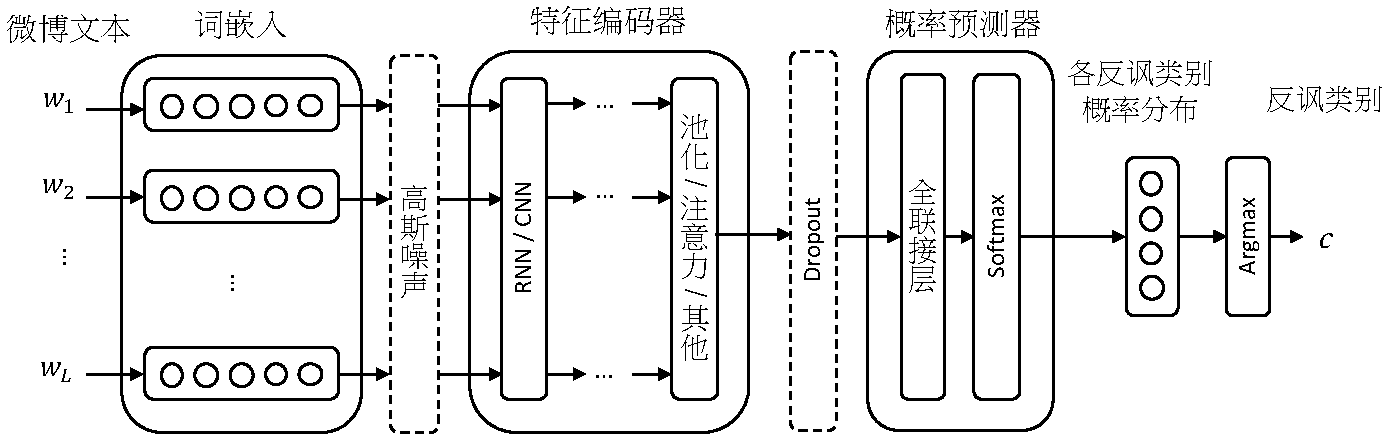
\includegraphics[width=\textwidth]{img/irony_det_cls_framework.pdf}
  \caption{反讽识别子分类器模型框架}
  \label{fig:irony_det_cls_framework}
\end{figure}

第二部分是分析我们设计的识别系统的性能。我们会观察每一轮决策的调整如何改变局部的预测结果,而这些局部变化如何影响系统的整体性能。另外我们也会透过对设计的系统框架进行修改和比较,分析设计的合理性,以及当尝试将这种识别系统设计方式应用到其他场景时有哪些细节值得注意。

按照国际比赛SemEval-2018任务三的设置,各个任务均以F1值作为识别系统性能的主要评价指标。对于其中一个类别$c$的F1值,其定义如下:

\begin{align}
  F_c = \frac{2 \times P_c \times R_c}{P_c + R_c} 
\end{align}

其中 $P_c$ 为类别$c$的正确率,$R_A$ 为类别$c$的召回率,其定义如下:

\begin{align}
  P_c &= \frac{TP_c}{TP_c + FP_c} \\
  R_c &= \frac{TP_c}{TP_c + FN_c}
\end{align} 

其中$TP_c$表示被系统预测为类别$c$,且真实标签为类别$c$的样本数量;$FP_c$表示被系统预测为类别$c$,但真实标签不是类别$c$的样本数量;$FN_c$被系统预测为不是类别$c$,但真实标签为类别$c$的样本数量。对于子任务一,系统性能以“带有反讽”一类样本的F1值为主要评估指标。对于子任务二,系统性能以各个类别的F1值的宏平均作为主要评价指标,即:

\begin{align}
  macro-F1 = \sum\limits_{c \in C}F_c
\end{align}

此处$C$对应子任务二中四个类别组成的集合,即\{没有反讽,基于相反语义的反讽,情景反讽,其他反讽\}。在以下实验中,我们除了观察F1值、正确率和召回率,我们还会给出模型的准确率,其定义如下:

\begin{align}
  Acc &= \frac{\sum\limits_{c \in C} TP_c}{\sum\limits_{c \in C}(TP_c + FP_c)}
\end{align}

其中$TP_c$和$FP_c$如前述的定义,而$C$在子任务一中对应两个类别组成的集合,即\{没有反讽,带有反讽\}。

\subsection{模型训练}

对于不同的模型,我们都采用了以下策略来进行训练:

\begin{itemize}

\item 对于每个子分类器,在训练开始前我们先从每一类的训练样本中随机选出10\%的样本作为验证集,以此保留各个类的样本量分布。在每一轮模型训练中,学习算法基于另外90\%的训练样本对网络参数进行调整,然后计算模型在验证集上的F1值,经过有限轮迭代后,取在验证集上达到最优F1值的网络参数作为该子分类器最终的参数,以此缓解在训练数据上过拟合的问题。另外由于最终预测结合由多个子分类器投票联合得出,为了充分运用训练数据,每个分类器的验证集为独立随机筛选得出,一方面保证每个训练样本都有概率被用于某个分类器的参数调整,另一方面使得各个分类器的训练数据不同,因此对文本特征的建模也会有所不同,理论上对过拟合同样有缓解的作用,更有利于最后的投票。

\item 对于词嵌入层,我们利用了章节\ref{ssec:embedding}中提到的Baziotis等人\cite{baziotis2018ntua}提供的词嵌入模型,直接用于初始化词嵌入层的参数。在训练过程中,我们不对词嵌入层的参数进行调整。考虑到若允许词嵌入层的参数调整,那么只有在训练集中出现过的词的词向量有机会被修改,词嵌入空间因此有所改动,只出现在验证集或测试集上的词的词向量在新的词嵌入空间中表达的意义就有可能出现偏差。另外对于词嵌入模型中未被覆盖的单词,若它在至少2个训练样本中出现,则为其随机生成词向量。

\item 在训练阶段中,我们在词嵌入层后添加高斯噪音。由于词嵌入算法在原理上使得意思相似的单词投影到词嵌入空间中距离相近的点上,高斯噪音的添加相当于把原本的单词替换成近义词,使得模型能更好地识别近义词构成的语言模式,另一方面缓解过拟合的问题。在验证和测试阶段,高斯躁音的标准方差被调整为零,即不起作用。

\item 在训练阶段中,我们在特征编码器和概率预测器之前添加了Dropout层,以概率$p_{Dropout}$将特征编码器得出特征向量上的各位数值置为零,并对没有被置零的各位数值乘以常量 $\frac{1}{1-p_{dropout}}$。在验证和测试阶段,Dropout层不起作用。

\item 在模型训练的损失函数,我们以权重$l_2$加入了概率预测器中全联接层的权重(不包括偏移量)的L2正则项。

\end{itemize}

\subsection{结果与分析}

pass

\begin{table}[htb]
  \centering
  \begin{minipage}[t]{0.8\linewidth}
  \caption{反讽识别子任务一子分类器性能}
  \label{tab:exp_irony_det_A_single_result}
    \begin{tabularx}{\linewidth}{X|cccc}
    \toprule[1.5pt]
    & 准确率 & 正确率 & 召回率 & F1值 \\
    \hline
    CNN + 最大池 & 0.6658 & 0.5548 & 0.7974 & 0.6544 \\ % A_cnn_ek_1553221371
    CNN + 注意力机制 & 0.6008 & 0.4980 & 0.8039 & 0.6150 \\  % A_cnn_ek_1554345958
    \hline
    GRU & 0.6607 & 0.5542 & 0.7395 & 0.6336 \\ % A_gru_ek_1553070254
    GRU + 注意力机制 & 0.6569 & 0.5482 & 0.7685 & 0.6399 \\ % A_gru_ek_1553074900
    \hline
    BiGRU & 0.6594 & 0.5534 & 0.7331 & 0.6307 \\ % A_bgru_ek_1553075855
    BiGRU + 注意力机制 & 0.6582 & 0.5473 & 0.8006 & 0.6501 \\ % A_bgru_ek_1553068355
    \hline
    LSTM & 0.6390 & 0.5276 & \bf 0.8617 & 0.6545 \\ % A_lstm_ek_1553071939
    LSTM + 注意力机制 & 0.6862 & 0.5768 & 0.7846 & 0.6640 \\ % A_lstm_ek_1553075765
    \hline
    BiLSTM & 0.6798 & 0.5721 & 0.7653 & 0.6547 \\ % A_blstm_ek_1553075473
    BiLSTM + 注意力机制 & \bf 0.6888 & 0.5861 & 0.7331 & 0.6514 \\ % A_blstm_ek_1553583756
    2层BiLSTM & 0.6709 & 0.5577 & 0.8232 & \bf 0.6649 \\ % A_nblstm_ek_1554346535
    2层BiLSTM + 注意力机制 & \bf 0.6888 & \bf 0.5870 & 0.7267 & 0.6494 \\ % A_nblstm_ek_1554346515
    \bottomrule[1.5pt]
    \end{tabularx}
  \end{minipage}
\end{table}

\begin{table}[htb]
  \centering
  \begin{minipage}[t]{0.9\linewidth}
  \caption{反讽识别子任务一前五名参赛系统性能}
  \label{tab:exp_irony_det_A_other_comp}
    \begin{tabularx}{\linewidth}{c|X|cccc}
    \toprule[1.5pt]
    排名 & 队伍名称 & 准确率 & 正确率 & 召回率 & F1值 \\
    \hline 
    1 & THU\_NGN & \bf 0.7347 & 0.6304 & 0.8006 & \bf 0.7054 \\
    2 & NTUA-SLP & 0.7321 & \bf 0.6535 & 0.6913 & 0.6719 \\
    3 & WLV & 0.6429 & 0.5317 & \bf 0.8360 & 0.6500 \\
    4 & (无) & 0.6607 & 0.5506 & 0.7878 & 0.6481 \\
    5 & NIHRIO, NCL & 0.7015 & 0.6091 & 0.6913 & 0.6476 \\
    \hline 
    & 我们的系统 & 0.7258 & 0.6176 & 0.8103  & 0.7010 \\
    \bottomrule[1.5pt]
    \end{tabularx}
  \end{minipage}
\end{table}

\begin{table}[htb]
  \centering
  \begin{minipage}[t]{0.8\linewidth}
  \caption{反讽识别子任务一子分类器性能}
  \label{tab:exp_irony_det_B_result}
    \begin{tabularx}{\linewidth}{X|cccc}
    \toprule[1.5pt]
    & 准确率 & 正确率 & 召回率 & F1值 \\
    \hline
    CNN & 0.6531 & \bf 0.5090 & 0.4667 & 0.4432 \\ % B_cnn_ek_1554446864
    CNN + 注意力机制 & 0.6186 & 0.4467 & 0.4214 & 0.4030 \\ % B_cnn_ek_1554446879
    \hline
    GRU & 0.6148 & 0.4437 & 0.4693 & 0.4476 \\ % B_gru_ek_1554447274
    GRU + 注意力机制 & 0.6531 & 0.4253 & 0.4605 & 0.4370 \\ % B_gru_ek_1554447525
    \hline
    BiGRU & \bf 0.6722 & 0.4868 & 0.4779 & \bf 0.4768 \\ % B_bgru_ek_1554447516
    BiGRU + 注意力机制 & 0.6301 & 0.4543 & 0.4638 & 0.4497 \\ % B_bgru_ek_1554447697
    \hline
    LSTM & 0.6186 & 0.4313 & 0.4490 & 0.4307 \\ % B_lstm_ek_1554447721
    LSTM + 注意力机制 & 0.6416 & 0.4046 & 0.4394 & 0.4148 \\ % B_lstm_ek_1554447878
    \hline
    BiLSTM & 0.6582 & 0.4875 & 0.4537 & 0.4447 \\ % B_blstm_ek_1554447955
    BiLSTM+att & 0.6352 & 0.4168 & 0.4386 & 0.4160 \\ % B_blstm_ek_1554448216
    \hline
    2层BiLSTM & 0.6582 & 0.5068 & 0.4762 & 0.4644 \\ % B_nblstm_ek_1554448237
    2层BiLSTM + 注意力机制 & 0.6314 & 0.4824 & \bf 0.4864 & 0.4657 \\ % B_nblstm_ek_1554448594
    \bottomrule[1.5pt]
    \end{tabularx}
  \end{minipage}
\end{table}

\begin{table}[htb]
  \centering
  \begin{minipage}[t]{0.8\linewidth}
  \caption{反讽识别子任务一子分类器性能}
  \label{tab:exp_irony_det_Bb01_result}
    \begin{tabularx}{\linewidth}{X|cccc}
    \toprule[1.5pt]
    & 准确率 & 正确率 & 召回率 & F1值 \\
    \hline
    CNN & 0.7991 & 0.7438 & 0.7791 & 0.7562 \\ % Bb01_cnn_ek_1554448736
    CNN + 注意力机制 & 0.6829 & 0.6494 & 0.6909 & 0.6470 \\ % Bb01_cnn_ek_1554448788
    \hline
    GRU & 0.8100 & \bf 0.7566 & 0.7944 & 0.7699 \\ % Bb01_gru_ek_1554448924
    GRU + 注意力机制 & 0.7677 & 0.7196 & 0.7679 & 0.7303 \\ % Bb01_gru_ek_1554449053
    \hline
    BiGRU & 0.8085 & 0.7565 & \bf 0.7993 & 0.7705 \\ % Bb01_bgru_ek_1554449115
    BiGRU + 注意力机制 & 0.7425 & 0.3713 & 0.5000 &  0.4261 \\ % Bb01_bgru_ek_1554449693
    \hline
    LSTM & 0.8053 & 0.7525 & 0.7932 & 0.7661 \\ % Bb01_lstm_ek_1554449707
    LSTM + 注意力机制 & \bf 0.8257 & 0.7717 & 0.7791 & \bf 0.7752 \\ % Bb01_lstm_ek_1554449864
    \hline
    BiLSTM & 0.7551 & 0.7169 & 0.7734 & 0.7236 \\ % Bb01_blstm_ek_1554449881
    BiLSTM + 注意力机制 & 0.7174 & 0.6909 & 0.7460 & 0.6889 \\ % Bb01_blstm_ek_1554450198
    \hline
    2层BiLSTM & 0.7849 & 0.7339 & 0.7795 & 0.7465 \\ % Bb01_nblstm_ek_1554450231
    2层BiLSTM + 注意力机制 & 0.7928 & 0.7421 & 0.7888 & 0.7554 \\ % Bb01_nblstm_ek_1554450448
    \bottomrule[1.5pt]
    \end{tabularx}
  \end{minipage}
\end{table}

\begin{table}[htb]
  \centering
  \begin{minipage}[t]{0.8\linewidth}
  \caption{反讽识别子任务一子分类器性能}
  \label{tab:exp_irony_det_Bb02_result}
    \begin{tabularx}{\linewidth}{X|cccc}
    \toprule[1.5pt]
    & 准确率 & 正确率 & 召回率 & F1值 \\
    \hline
    CNN & \bf 0.8656 & \bf 0.7634 & 0.6167 & 0.6473 \\ % Bb02_cnn_ek_1554450719
    CNN + 注意力机制 & 0.8477 & 0.6865 & 0.5917 & 0.6117 \\ % Bb02_cnn_ek_1554450772
    \hline
    GRU & 0.8495 & 0.6942 & 0.6024 & 0.6242 \\ % Bb02_gru_ek_1554450862
    GRU + 注意力机制 & 0.8333 & 0.6708 & 0.6556 & 0.6625 \\ % Bb02_gru_ek_1554451013
    \hline
    BiGRU & 0.8423 & 0.6645 & 0.5789 & 0.5951 \\ % Bb02_bgru_ek_1554451047
    BiGRU + 注意力机制 & 0.8423 & 0.6825 & 0.6416 & 0.6572 \\ % Bb02_bgru_ek_1554451155
    \hline
    LSTM & 0.8513 & 0.7027 & 0.6372 & 0.659 \\ % Bb02_lstm_ek_1554451286
    LSTM + 注意力机制 & 0.8387 & 0.6676 & 0.6153 & 0.6325 \\ % Bb02_lstm_ek_1554451194
    \hline
    BiLSTM & 0.8351 & 0.6575 & 0.6084 & 0.6243 \\ % Bb02_blstm_ek_1554451336
    BiLSTM + 注意力机制 & 0.8369 & 0.6797 & 0.6674 & 0.6731 \\ % Bb02_blstm_ek_1554451401
    \hline
    2层BiLSTM & 0.8262 & 0.6691 & 0.6803 & 0.6743 \\ % Bb02_nblstm_ek_1554451496
    2层BiLSTM + 注意力机制 & 0.8513 & 0.7076 & \bf 0.6806 & \bf 0.6924 \\ % Bb02_nblstm_ek_1554451575
    \bottomrule[1.5pt]
    \end{tabularx}
  \end{minipage}
\end{table}

\begin{table}[htb]
  \centering
  \begin{minipage}[t]{0.8\linewidth}
  \caption{反讽识别子任务一子分类器性能}
  \label{tab:exp_irony_det_Bb03_result}
    \begin{tabularx}{\linewidth}{X|cccc}
    \toprule[1.5pt]
    & 准确率 & 正确率 & 召回率 & F1值 \\
    \hline
    CNN & \bf 0.8860 & \bf 0.7123 & \bf 0.5781 & \bf 0.6016 \\ % Bb03_cnn_ek_1553500286
    CNN + 注意力机制 & 0.7981 & 0.493 & 0.4934 & 0.4932 \\ % Bb03_cnn_ek_1554453416
    \hline
    GRU & 0.8336 & 0.5873 & 0.5836 & 0.5853 \\ % Bb03_gru_ek_1554452318
    GRU + 注意力机制 & 0.8841 & 0.6928 & 0.5070 &  0.4848 \\ % Bb03_gru_ek_1554452300
    \hline
    BiGRU & 0.8411 & 0.5481 & 0.5317 & 0.5353 \\ % Bb03_bgru_ek_1554452373
    BiGRU + 注意力机制 & 0.8822 & 0.4419 & 0.4989 & 0.4687 \\ % Bb03_bgru_ek_1554452659
    \hline
    LSTM & 0.8486 & 0.5603 & 0.5360 & 0.5409 \\ % Bb03_lstm_ek_1554452412
    LSTM + 注意力机制 & 0.8841 & 0.4421 & 0.5000 & 0.4692 \\ % Bb03_lstm_ek_1554452800
    \hline
    BiLSTM & 0.8430 & 0.5663 & 0.5468 & 0.5527 \\ % Bb03_blstm_ek_1554452497
    BiLSTM + 注意力机制 & 0.8822 & 0.4419 & 0.4989 & 0.4687 \\ % Bb03_blstm_ek_1554452804
    \hline
    2层BiLSTM & 0.8355 & 0.5483 & 0.5356 & 0.5393 \\ % Bb03_nblstm_ek_1554452506
    2层BiLSTM + 注意力机制 & 0.7944 & 0.4571 & 0.4633 & 0.4600 \\ % Bb03_nblstm_ek_1554452977
    \bottomrule[1.5pt]
    \end{tabularx}
  \end{minipage}
\end{table}

\begin{table}[htb]
  \centering
  \begin{minipage}[t]{0.7\linewidth}
  \caption{反讽识别子任务二多步决策后的识别性能}
  \label{tab:exp_irony_det_B_ensemble_result}
    \begin{tabularx}{\linewidth}{X|XXXX}
    \toprule[1.5pt]
    & 准确率 & 正确率 & 召回率 & F1值 \\
    \hline
    第一轮 & \bf 0.6837 & \bf 0.5512 & 0.5016 & 0.5253 \\
    第二轮 & 0.6811 & 0.5464 & 0.5113 & 0.5282 \\
    第三轮 & 0.6786 & 0.5361 & 0.5498 & 0.5429 \\ 
    第四轮 & 0.6824 & 0.5443 & \bf 0.5531 & \bf 0.5486 \\
    \bottomrule[1.5pt]
    \end{tabularx}
  \end{minipage}
\end{table}

\begin{table}[htb]
  \centering
  \begin{minipage}[t]{0.8\linewidth}
  \caption{反讽识别子任务二前五名参赛系统性能}
  \label{tab:exp_irony_det_B_other_comp}
    \begin{tabularx}{\linewidth}{c|X|cccc}
    \toprule[1.5pt]
    排名 & 队伍名称 & 准确率 & 正确率 & 召回率 & F1值 \\
    \hline 
    1 & (无) & \bf 0.7321 & \bf 0.5768 & 0.5044 & 0.5074 \\
    2 & NTUA-SLP & 0.6518 & 0.4959 & 0.5124 & 0.4959 \\
    3 & THU\_NGN & 0.6046 & 0.4860 & 0.5414 & 0.4947 \\
    4 & (无) & 0.6033 & 0.4660 & 0.5058 & 0.4743 \\
    5 & NIHRIO, NCL & 0.6594 & 0.5446 & 0.4475 & 0.4437 \\
    \hline
    & 我们的系统 & 0.6824 & 0.5443 & \bf 0.5531 & \bf 0.5486 \\
    \bottomrule[1.5pt]
    \end{tabularx}
  \end{minipage}
\end{table}

% b03需要用class_weight

% \subsection{错误分析}

\section{本章小结}

pass

